%%%%%%%%%%%%%%%%%%%%%%%%%%%%%%%%%%%%%%%%%
% University/School Laboratory Report
% LaTeX Template
% Version 3.1 (25/3/14)
%
% This template has been downloaded from:
% http://www.LaTeXTemplates.com
%
% Original author:
% Linux and Unix Users Group at Virginia Tech Wiki 
% (https://vtluug.org/wiki/Example_LaTeX_chem_lab_report)
%
% License:
% CC BY-NC-SA 3.0 (http://creativecommons.org/licenses/by-nc-sa/3.0/)
%
%%%%%%%%%%%%%%%%%%%%%%%%%%%%%%%%%%%%%%%%%

%----------------------------------------------------------------------------------------
%	PACKAGES AND DOCUMENT CONFIGURATIONS
%----------------------------------------------------------------------------------------

\documentclass{article}

\usepackage{graphicx} % Required for the inclusion of images
\usepackage{natbib} % Required to change bibliography style to APA
\usepackage{amsmath} % Required for some math elements
\usepackage{mathtools}
\usepackage[export]{adjustbox}
\usepackage{subcaption}
\usepackage{float}
\usepackage{listings}
\usepackage{minted}

\DeclarePairedDelimiter{\abs}{\lvert}{\rvert}
\setlength\parindent{0pt} % Removes all indentation from paragraphs

\renewcommand{\labelenumi}{\alph{enumi}.} % Make numbering in the enumerate environment by letter rather than number (e.g. section 6)

%\usepackage{times} % Uncomment to use the Times New Roman font

%----------------------------------------------------------------------------------------
%	DOCUMENT INFORMATION
%----------------------------------------------------------------------------------------

\title{ECE 637 Digital Image Processing Laboratory: \\ 2-D Random Processes} % Title

\author{Yang \textsc{Wang}} % Author name

\date{\today} % Date for the report

\begin{document}

\maketitle % Insert the title, author and date

% If you wish to include an abstract, uncomment the lines below
% \begin{abstract}
% Abstract text
% \end{abstract}

% If you have more than one objective, uncomment the below:
%\begin{description}
%\item[First Objective] \hfill \\
%Objective 1 text
%\item[Second Objective] \hfill \\
%Objective 2 text
%\end{description}

%\subsection{Definitions}
%\label{definitions}
%\begin{description}
%\item[Stoichiometry]
%The relationship between the relative quantities of substances taking part in a reaction or forming a compound, typically a ratio of whole integers.
%\item[Atomic mass]
%The mass of an atom of a chemical element expressed in atomic mass units. It is approximately equivalent to the number of protons and neutrons in the atom (the mass number) or to the average number allowing for the relative abundances of different isotopes. 
%\end{description} 

%----------------------------------------------------------------------------------------
%	SECTION 1
%----------------------------------------------------------------------------------------

\section{Power Spectral Density of an Image}

In this section, a gray scale image is analyzed for its power spectral density content.
Different window size is used to calculate the normailzed energy spectrum. In the last
section, a better spectral density analysis implemetation is realized by applying multiple
non-overlapping windows of the same size to the image.

\subsection{Plot grayscale image}
	\begin{description}
	\item[]
	Plot the given gray scale image in MATLAB.
		\begin{figure}[h]
			\begin{center}
				\includegraphics[width=0.9\textwidth]{gs\string_img_4g.png}
				\caption{img04g.tif}
			\end{center}
		\end{figure}
	\end{description}

\subsection{Plot power spectral density for different block sizes}
	\begin{description}
	\item[]
	From Figure 2b) and 2c), even with increased block sizes, the power spectrum estimates
	main noisy.
		\begin{figure}[h]
			\begin{subfigure}{0.55\textwidth}
				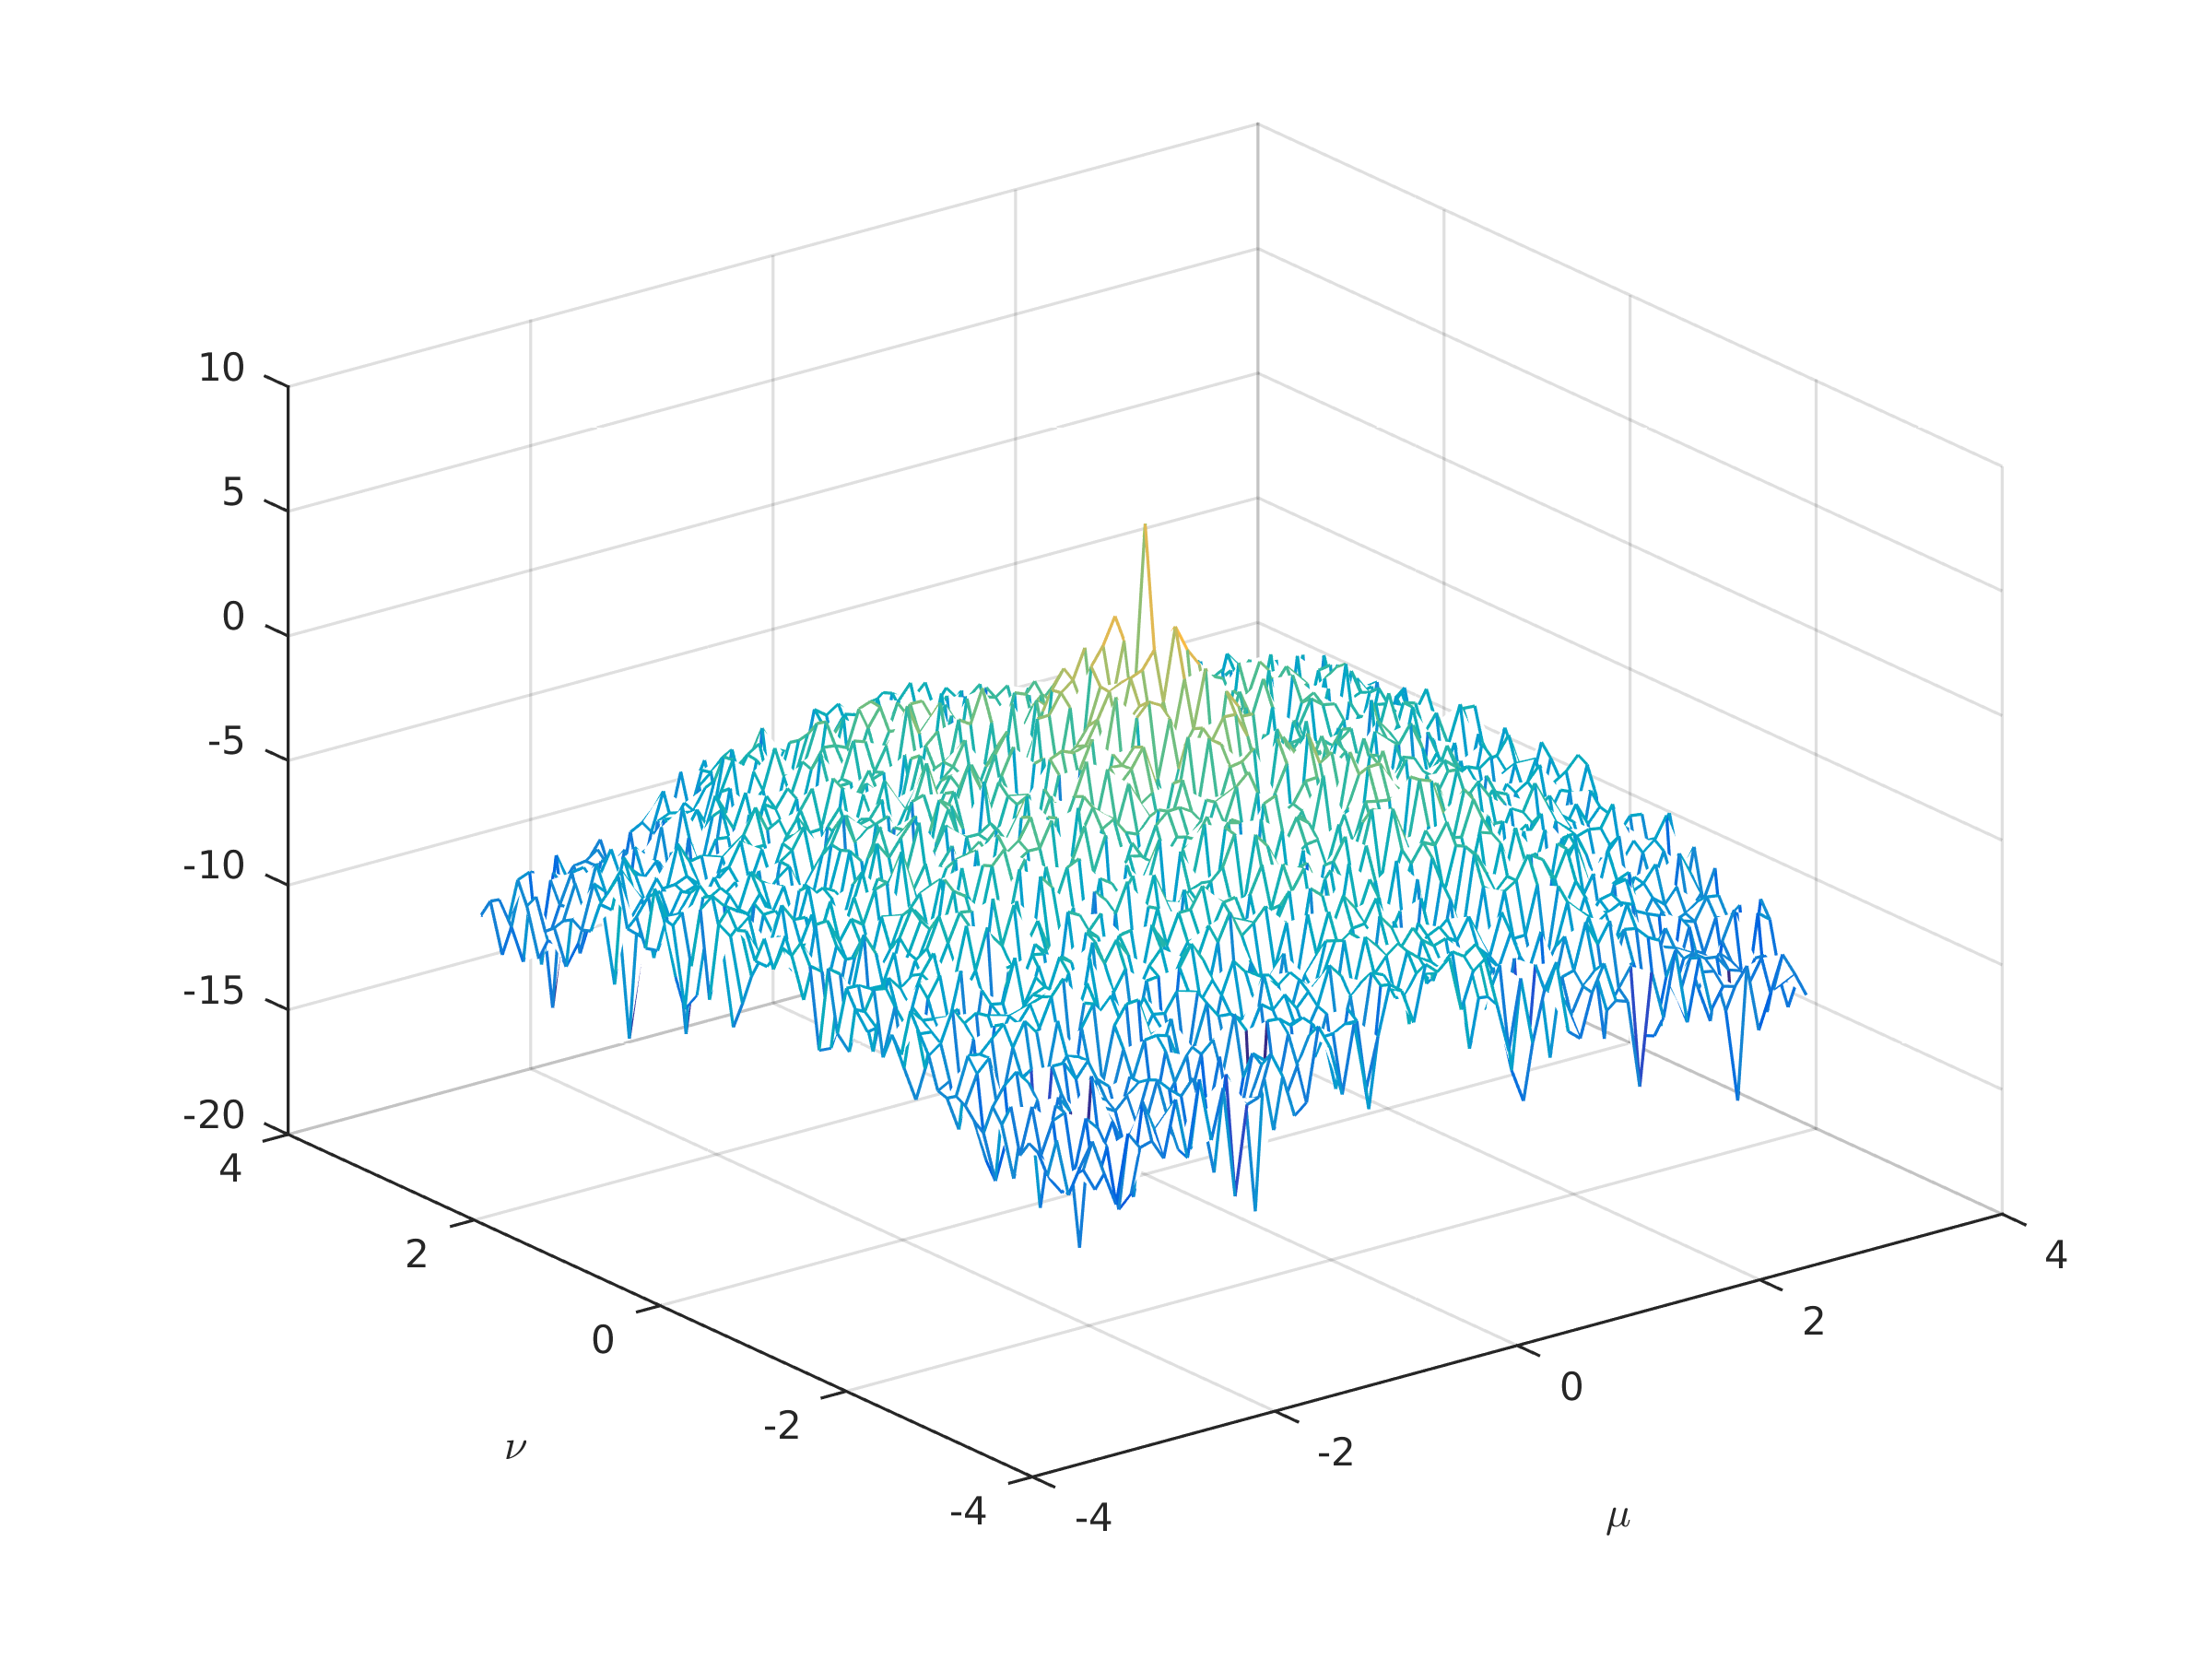
\includegraphics[width=0.9\linewidth, left]{psd_64x64.png} 
				\caption{PSD with block size 64$\times$64}
			\end{subfigure}
			\begin{subfigure}{0.55\textwidth}
				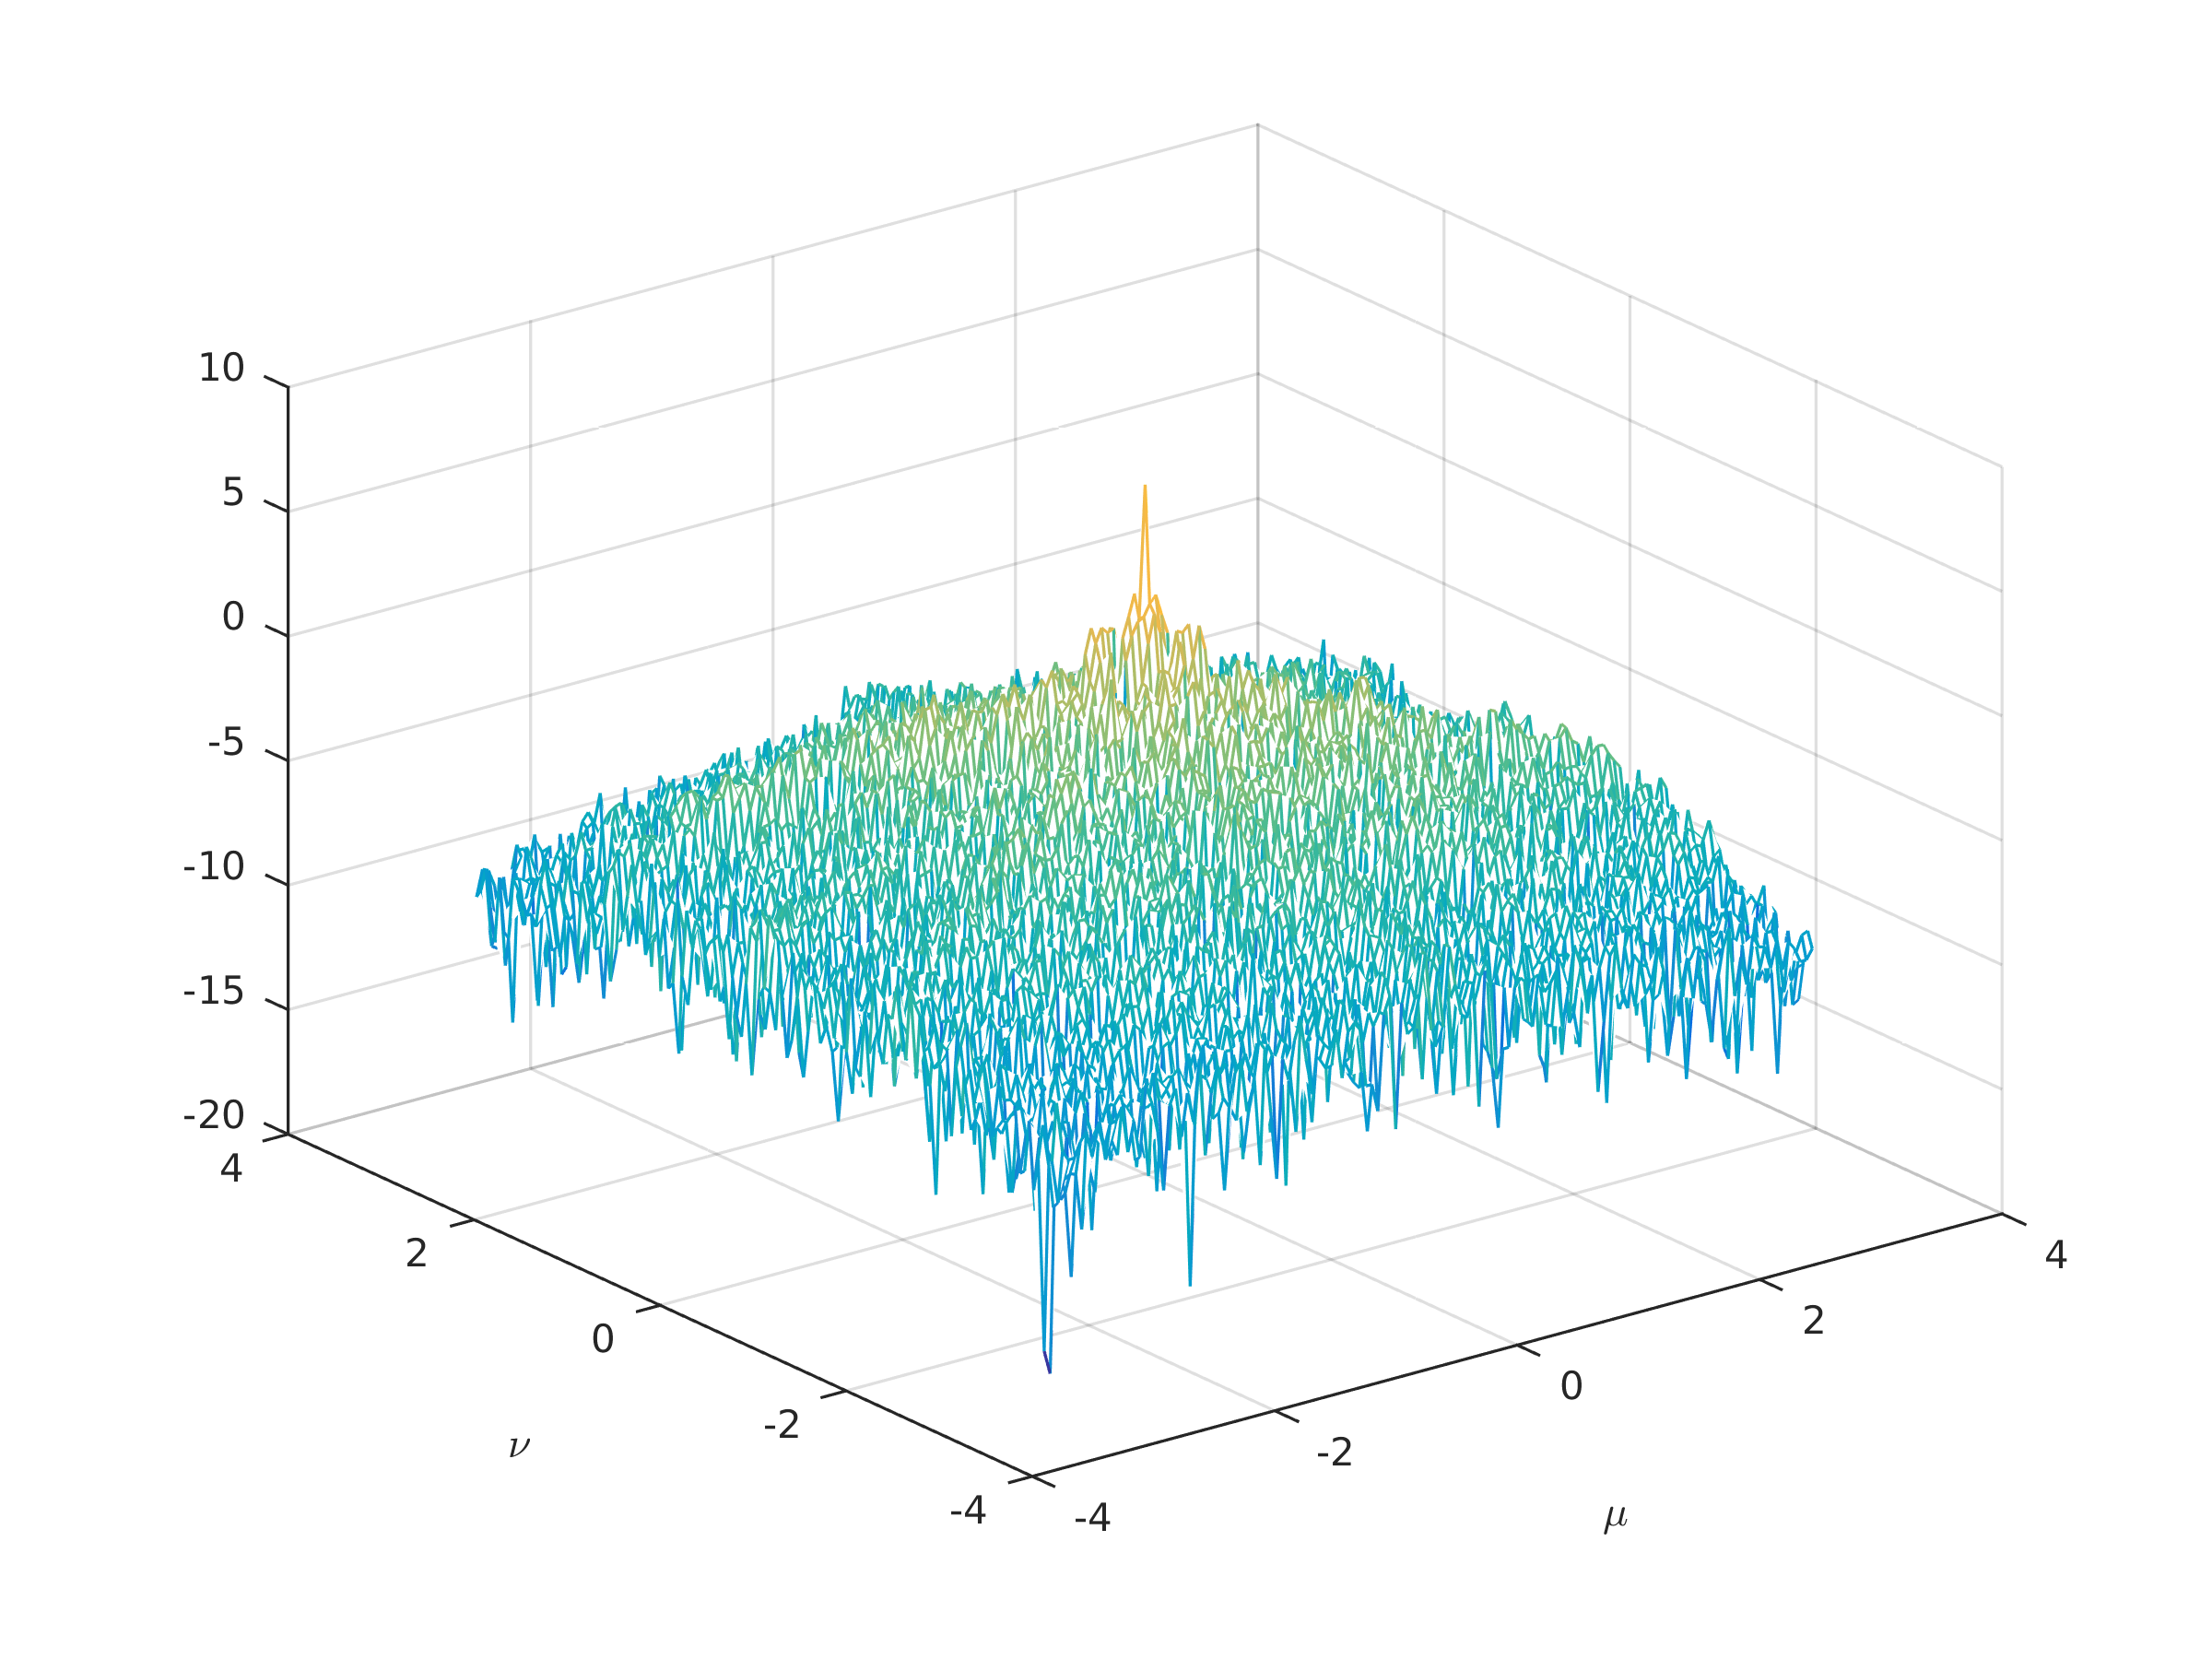
\includegraphics[width=0.9\linewidth, right]{psd_128x128.png}
				\caption{PSD with block size 128$\times$128}
			\end{subfigure}
			\begin{subfigure}{1.0\textwidth}
				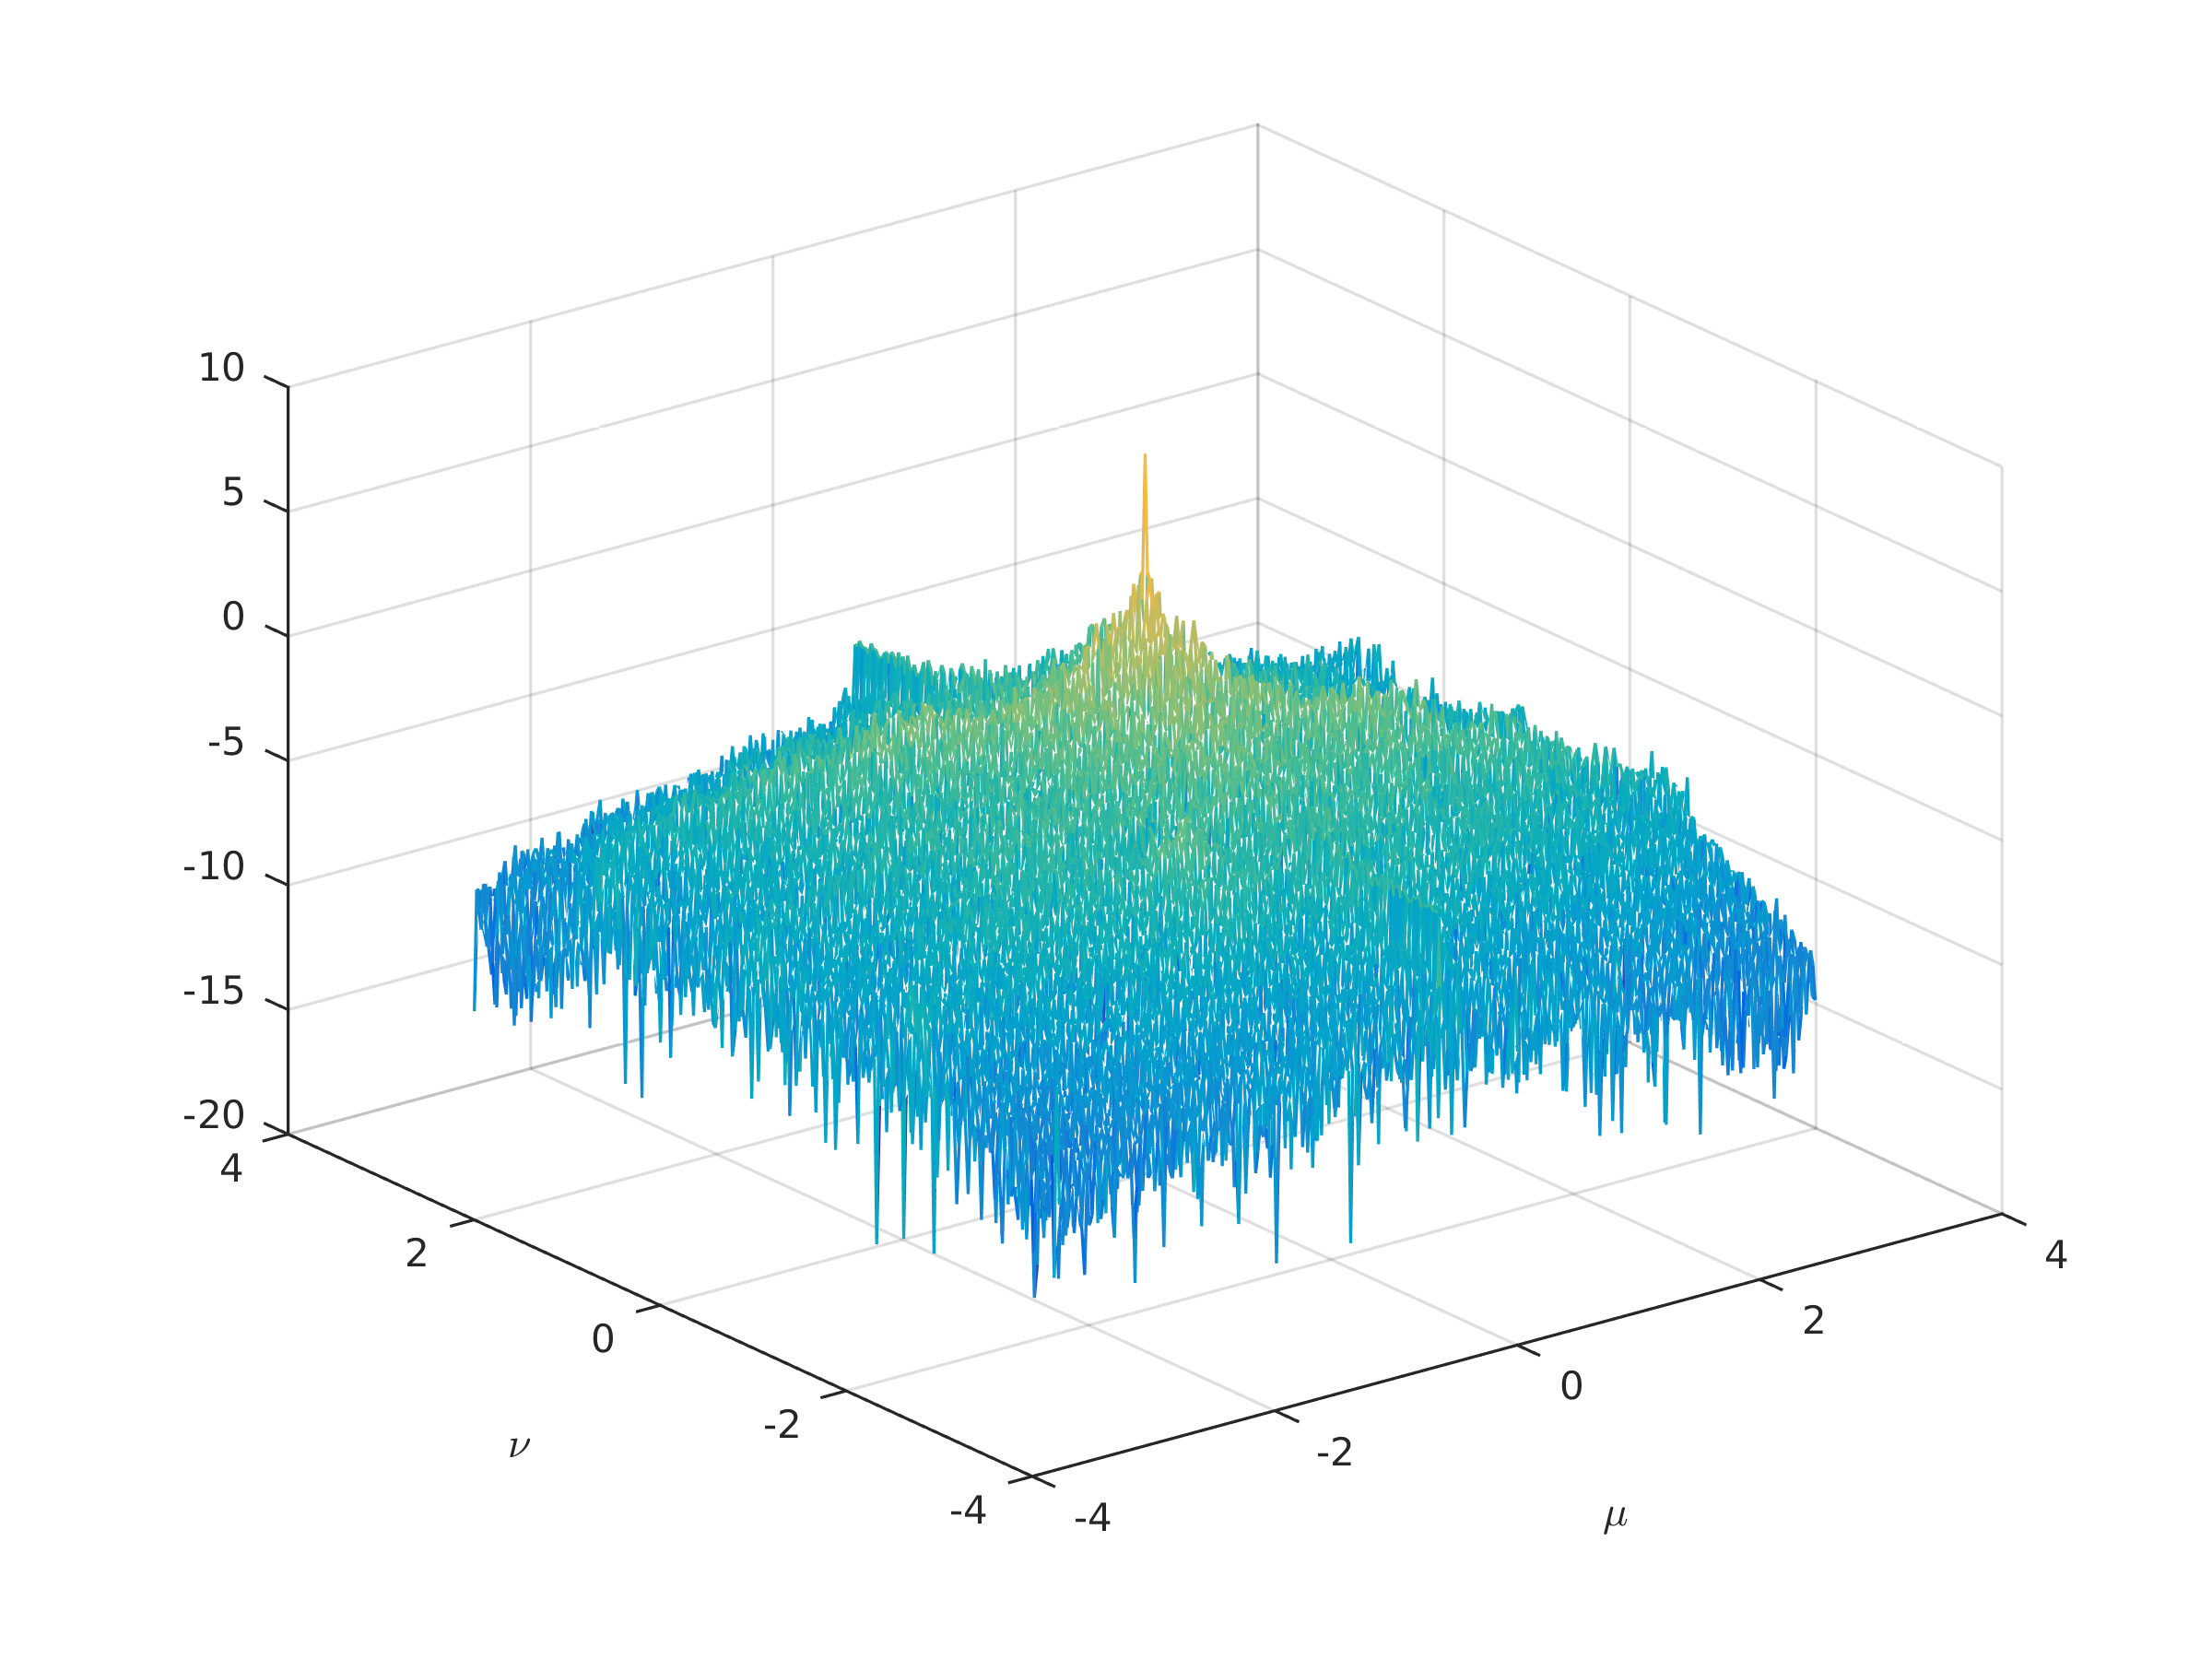
\includegraphics[width=0.6\linewidth, center]{psd_256x256.png}
				\caption{PSD with block size 256$\times$256}
			\end{subfigure}
			\caption{PSD with different block sizes}
		\end{figure}
	\end{description}

\pagebreak

\subsection{Plot improved power spectral density estimate}
	\begin{description}
	\item[]
	From Figure 3, the noise from the original PSD is eliminated.
		\begin{figure}[h]
			\begin{center}
				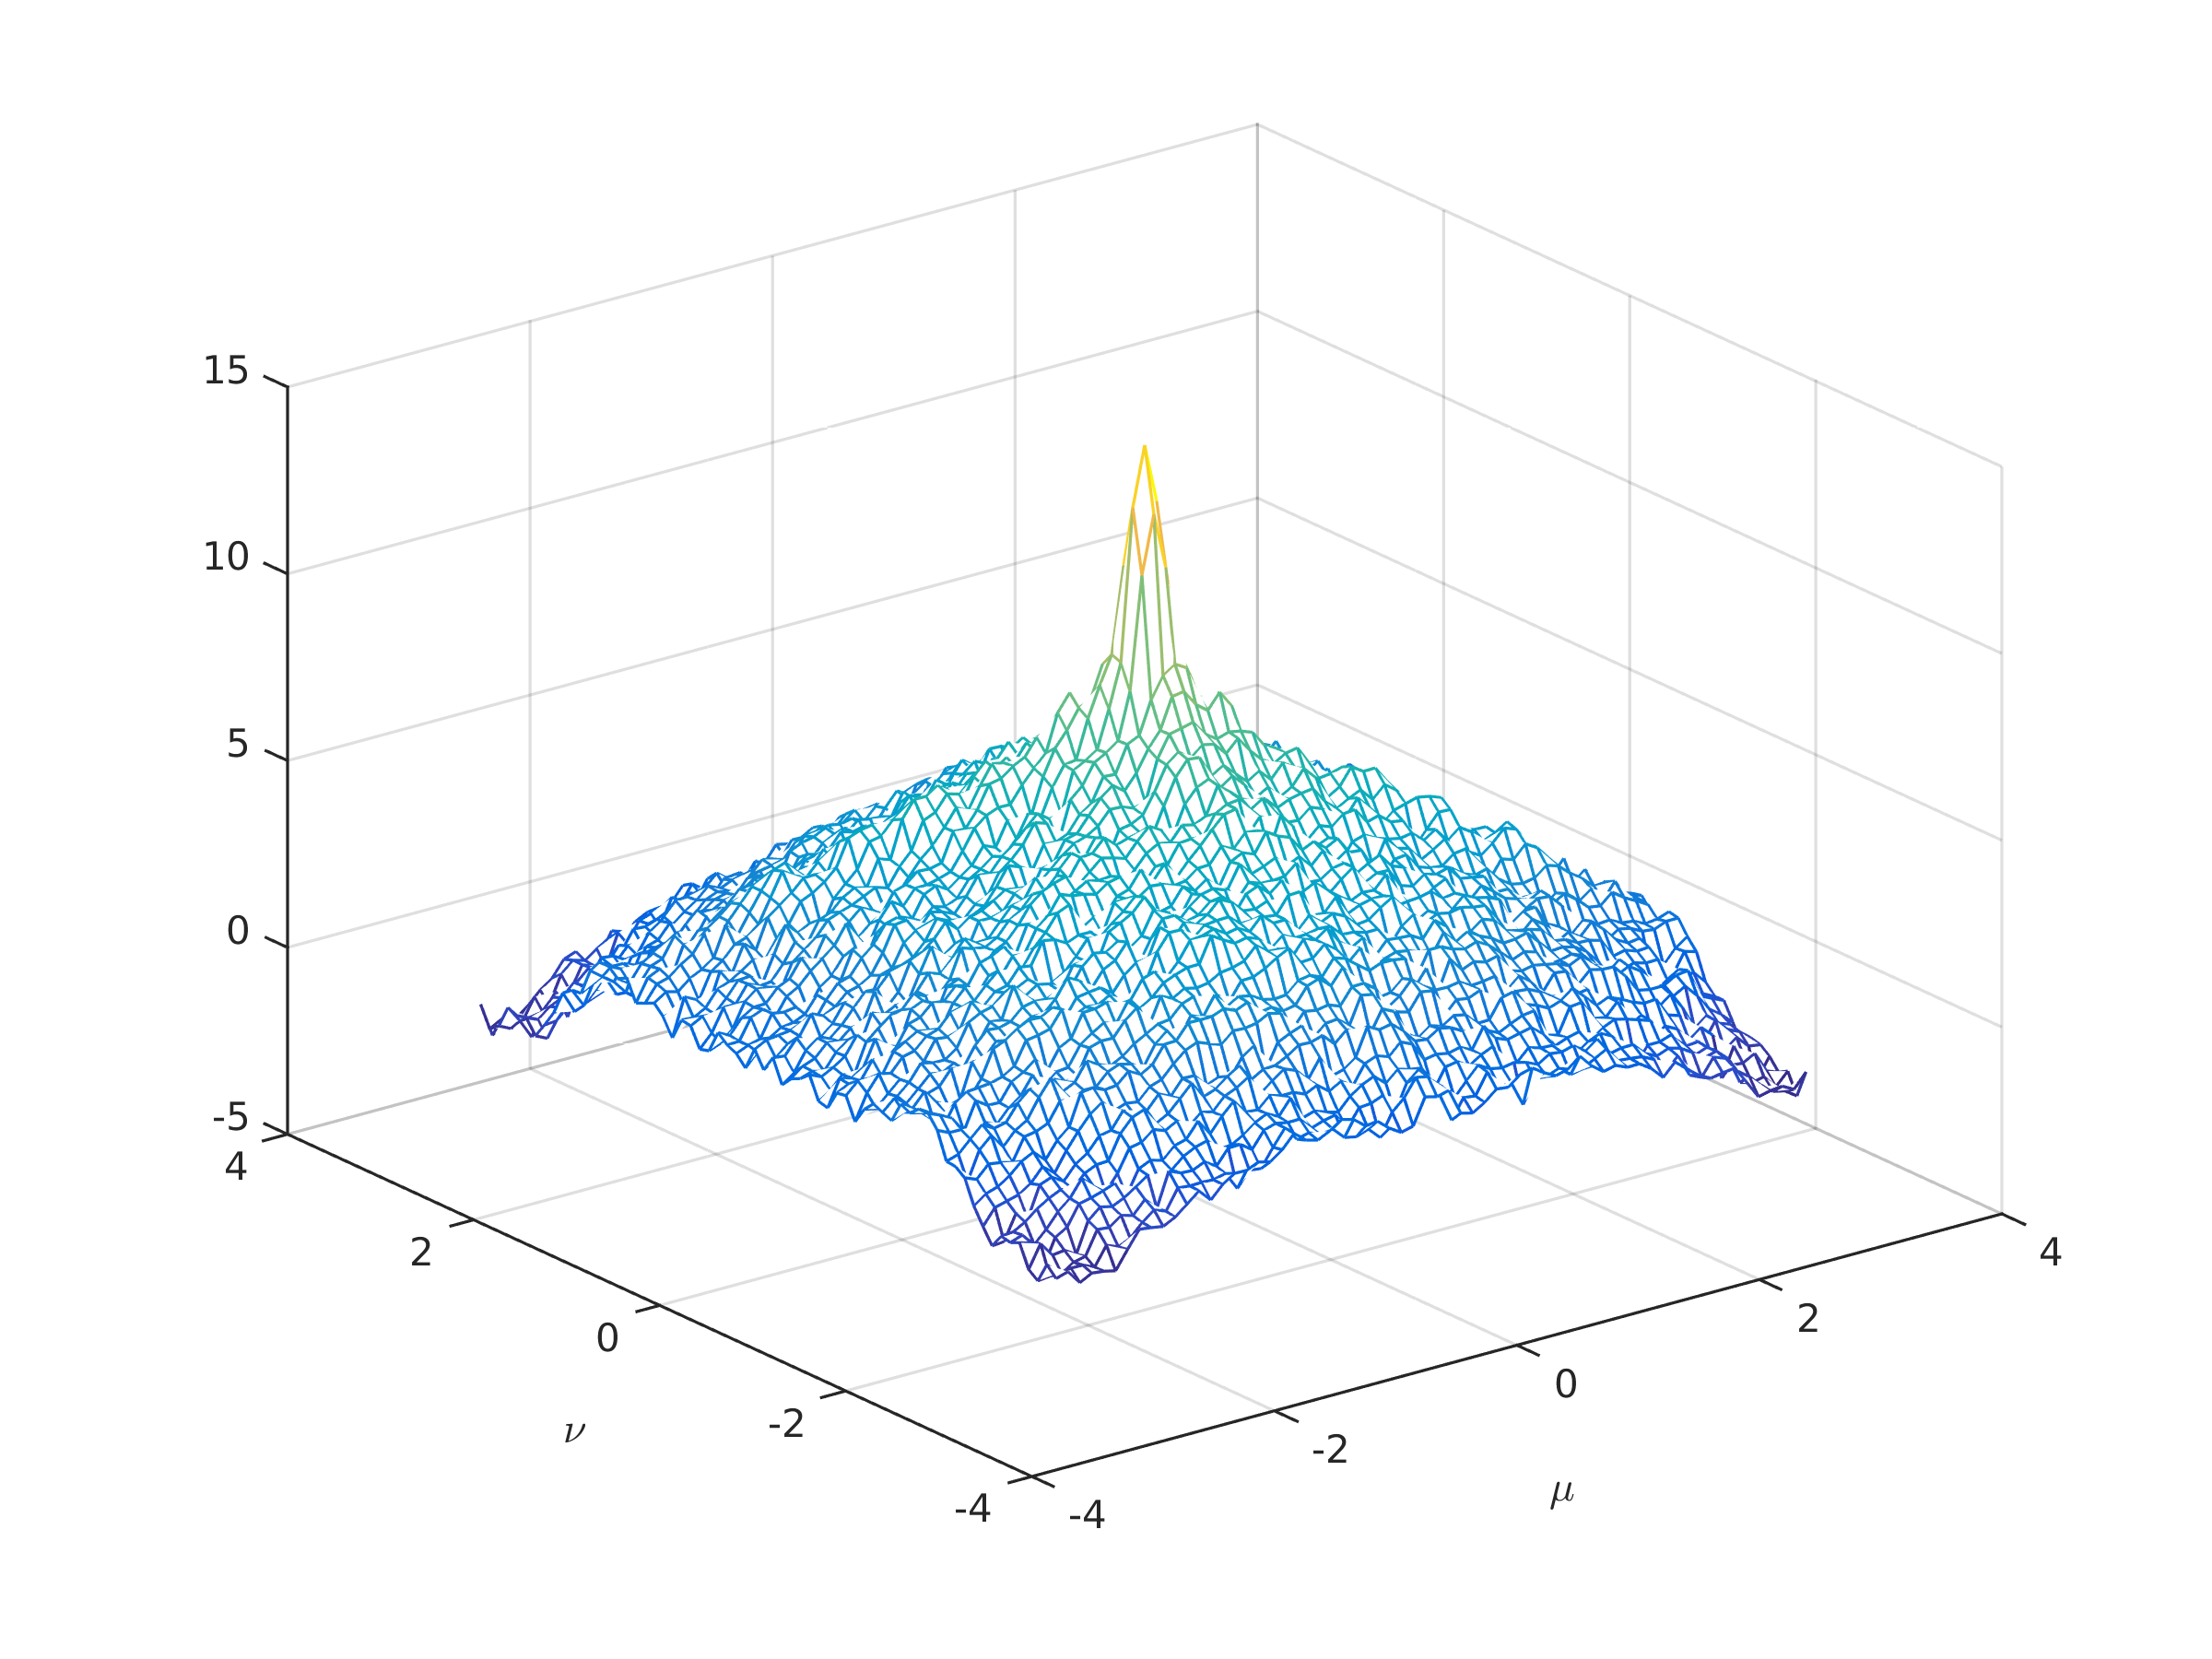
\includegraphics[width=0.9\textwidth]{psd_better.png}
				\caption{Improved PSD Estimate}
			\end{center}
		\end{figure}
	\end{description}

\subsection{Code listing}
	\subsubsection{BetterSpecAnal.m}
		\inputminted[tabsize=4,breaklines]{matlab}{BetterSpecAnal.m}

%----------------------------------------------------------------------------------------
%	SECTION 2
%----------------------------------------------------------------------------------------

\section{Power Spectral Density of a 2-D AR Process}
	In this section, a synthetic 2-D autoregressive (AR) process is generated and its
	power spectral density is analyzed.

\subsection{Plot the scaled image generated using rand()}
	\begin{description}
	\item[]
		\begin{figure}[h]
			\begin{center}
				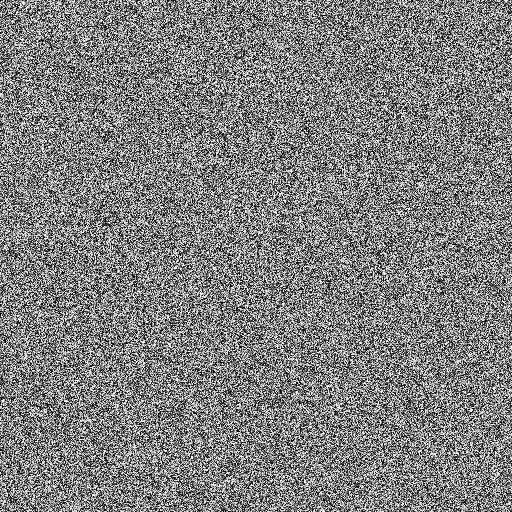
\includegraphics[width=0.7\textwidth]{randimg.png}
				\caption{Image generated using rand() uniformly distributed on \string[-0.5,0.5]}
			\end{center}
		\end{figure}
	\end{description}

\subsection{Find the difference equation to the given filter}
	\begin{description}
	\item[]
		We are given:
		\begin{equation}
			H(z_1,z_2) = \frac{3}{1-0.99z_1^{-1}-0.99z_2^{-1}+0.9801z_1^{-1}z_2^{-1}}
		\end{equation}
		We know,
		\begin{align*}
			H(z_1,z_2) = \frac{Y(z_1,z_2)}{X(z_1,z_2)}
		\end{align*}
		Hence,
		\begin{align*}
			Y(z_1,z_2) = 3X(z_1,z_2)+0.99z_1^{-1}Y(z_1,z_2)+0.99z_2^{-1}Y(z_1,z_2)-0.9801z_1^{-1}z_2^{-1}Y(z_1,z_2)
		\end{align*}
		Taking the inverse Z-transform,
		\begin{align*}
			y(m,n) = 3x(m,n)+0.99y(m-1,n)+0.99y(m,n-1)-0.9801y(m-1,n-1)
		\end{align*}
	\end{description}

\subsection{Plot the filtered image}
	\begin{description}
	\item[]
		\begin{figure}[h]
			\begin{center}
				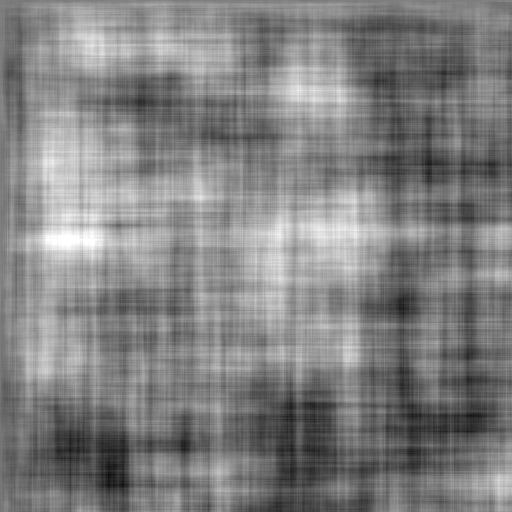
\includegraphics[width=0.7\textwidth]{randimg_f.png}
				\caption{Filtered results of noisy image}
			\end{center}
		\end{figure}
	\end{description}

\pagebreak

\subsection{Plot the theoretical result of log(PSD)}
	\subsubsection{Derivation of PSD}
		We know the relation:
		\begin{equation}
			S_y(e^{j\mu},e^{j\nu}) = \abs{H(e^{j\mu},e^{j\nu})}^{2}S_x(e^{j\mu},e^{j\nu})
		\end{equation}
		We need to derive the PSD of $\textit{x}$.
		We also know:
		\begin{align*}
			S_x(e^{j\mu},e^{j\nu}) = \lim_{N\to\infty}\frac{1}{N}E(\abs{X_N(e^{j\mu},e^{j\nu})}^{2})
		\end{align*}
		We have the relation:
		\begin{equation}
			Var[X] = E[X^{2}]-(E[X])^{2}
		\end{equation}
		For uniform distribution on interval [-0.5,0.5], $(E[X])^{2}=0$, hence,
		\begin{align*}
			Var[X] = E[X^{2}]
		\end{align*}
		Further,
		\begin{align*}
			S_x(e^{j\mu},e^{j\nu}) &= \lim_{N\to\infty}\frac{1}{N}E(\abs{X_N(e^{j\mu},e^{j\nu})}^{2}) \\
								   &= \lim_{N\to\infty}\frac{1}{N}NVar[X] \\
								   & = \sigma^{2} = \frac{1}{12}
		\end{align*}
		Therefore,
		\begin{align*}
			S_y(e^{j\mu},e^{j\nu}) &= \frac{1}{12}\abs{H(e^{j\mu},e^{j\nu})}^{2} \\
								   &= \frac{1}{12}\abs{\frac{3}{1-0.99z_1^{-1}-0.99z_2^{-1}+0.9801z_1^{-1}z_2^{-1}}}^{2}
		\end{align*}
	\pagebreak
	\subsubsection{Plot of theoretical PSD} 
		\begin{figure}[h]
			\begin{center}
				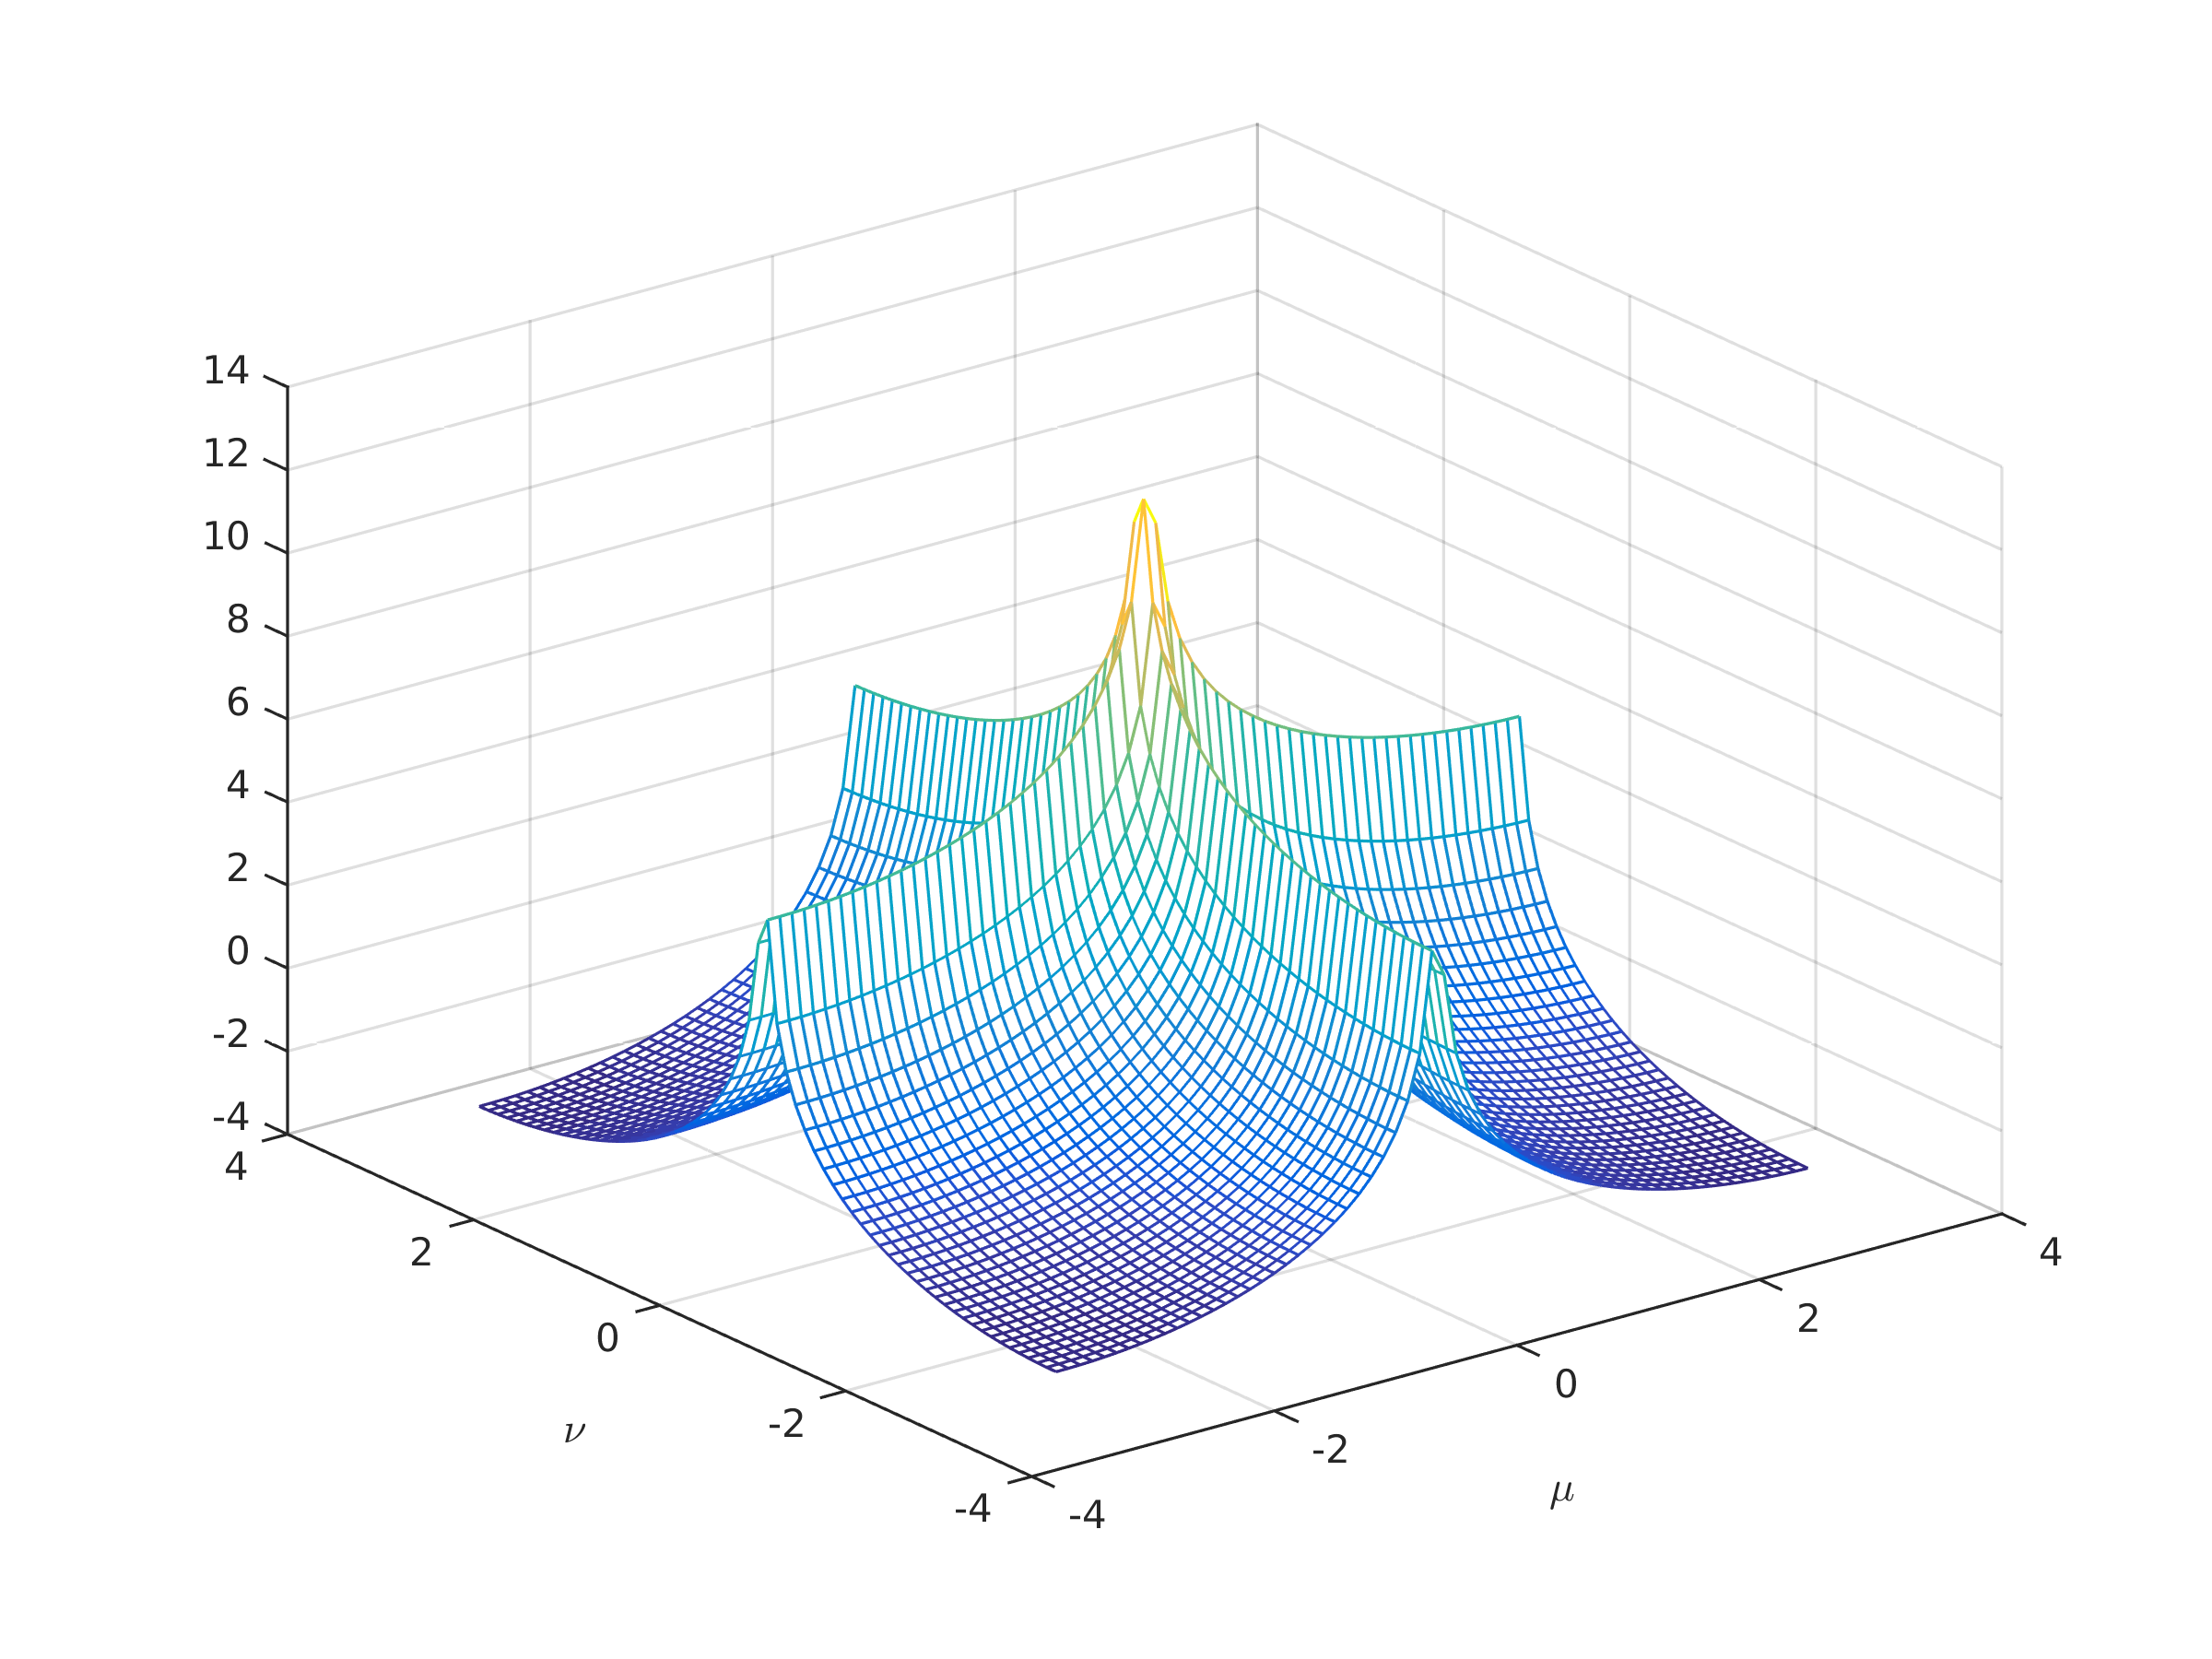
\includegraphics[width=0.6\textwidth]{psd_theo.png}
				\caption{Theoretical plot of PSD of 2-D AR Process}
			\end{center}
		\end{figure}

\subsection{Plot the estimated result of log(PSD)}
	\begin{description}
	\item[]
		\begin{figure}[h]
			\begin{center}
				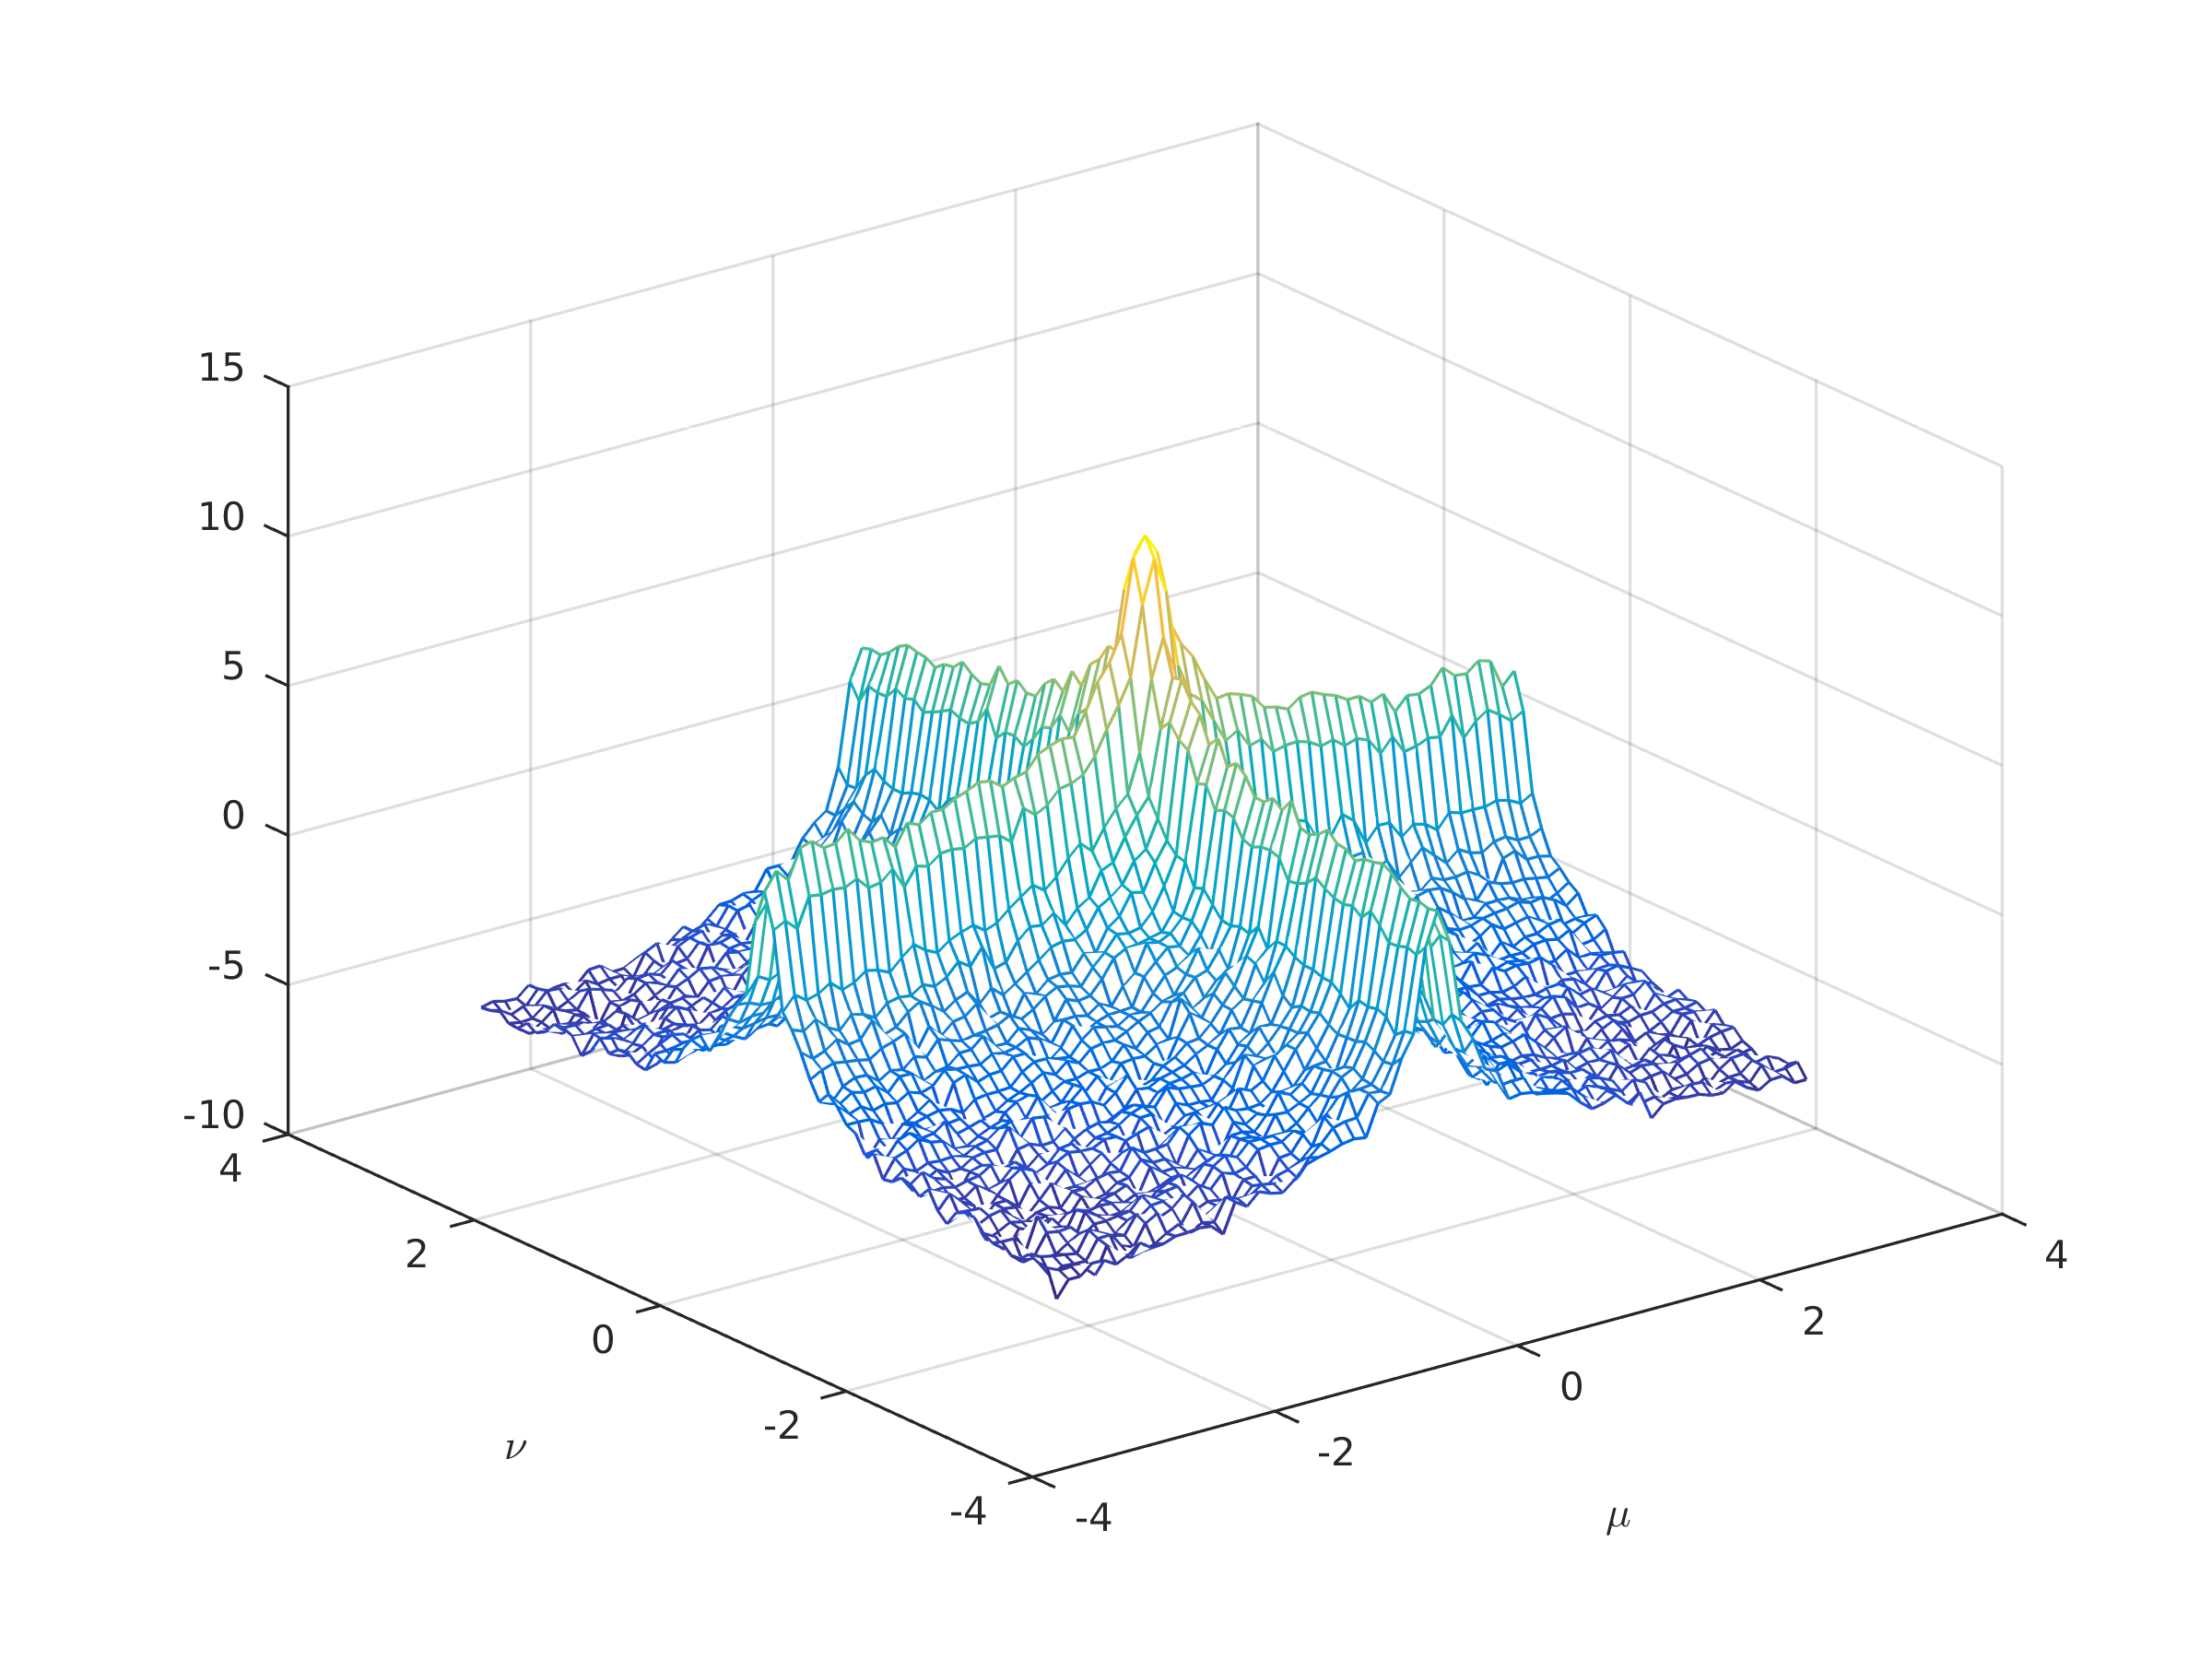
\includegraphics[width=0.6\textwidth]{psd_esti.png}
				\caption{Estimated plot of PSDi of 2-D AR Process}
			\end{center}
		\end{figure}
	\end{description}

\section{Additonal code listing}
	\subsection{SpecAnal.m}
		\inputminted[tabsize=4,breaklines]{matlab}{SpecAnal.m}

\end{document}
